\section{Problem Formulation and Motivation}
This section first formulates the problem in Section~2.1 and then presents key observations in Section~2.2. Finally, Section~2.3 discusses the main challenges in designing \system. The related terminologies are listed in Table~\ref{tab:symbols}.

\subsection{Problem Statement}

We begin with the standard Approximate Nearest Neighbor Search (ANNS) definition \cite{Song2025}.

\begin{table}[t]
  \caption{Summary of terminologies}
  \label{tab:symbols}
  \begin{tabular}{lp{6.3cm}}
    \toprule
    Symbol & Description\\
    \midrule
    $\mathcal{D}$ & Vector dataset. \\
    $\mathcal{D}_r$ & Vector dataset state after applying the batch updates at round $r$. \\
    % $\widehat{N}_k(q)$ & Approximate top-$k$ result set of query $q$. \\
    % $N_k^{\ast}(q)$ & Exact top-$k$ nearest-neighbor set of query $q$. \\
    $\mathrm{Recall@}k(q)$ & Recall of the approximate top-$k$ result for query $q$. \\
    $\mathcal{U}_r$ & Batch updates at round $r$. \\
    $\mathcal{Q}_r$ & Batch queries executed at round $r$. \\
	$R$ & The number of rounds we evaluate. \\
    $T_{\mathrm{search}}(q)$ & Search latency of query $q$. \\
    $T_{\mathrm{maintain}}(\mathcal{U}_r)$ & Maintenance time cost triggered by batch updates $\mathcal{U}_r$. \\
    $\mathrm{QPS}(R)$ & Average query throughput within $R$ rounds. \\
    $\tau$ & Tolerance threshold for Recall@$k$. \\
    \bottomrule
  \end{tabular}
\end{table}

\begin{figure*}
	\centering
	\subfloat[Top-$k$ overlap across rounds]{
		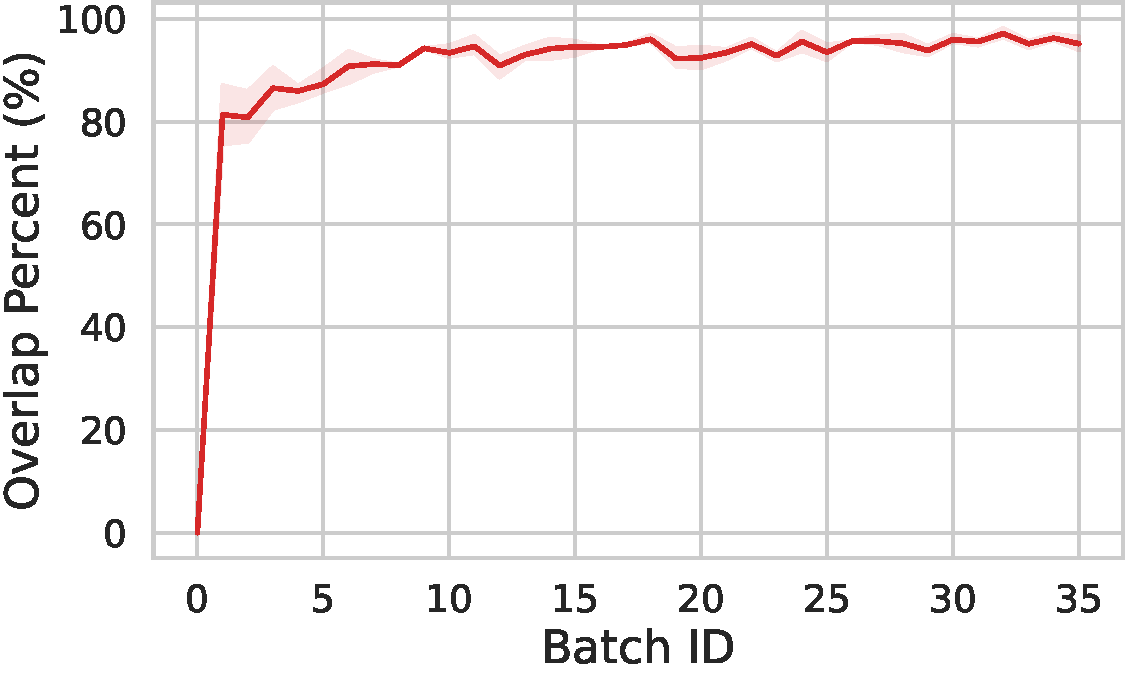
\includegraphics[width=0.57\columnwidth]{figures/repeat_topk_compare.pdf}
		\label{fig:repeat results}
	}\hspace{0.02\linewidth}
    \subfloat[Skewness of retrieved vector IDs]{
		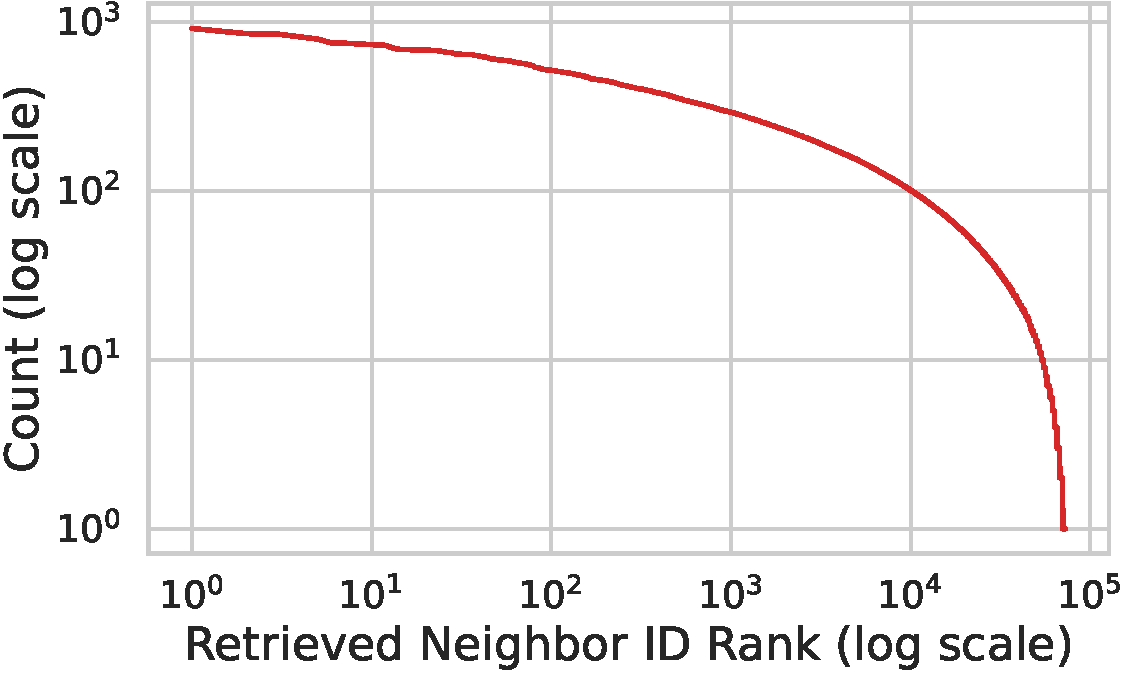
\includegraphics[width=0.57\columnwidth]{figures/rank_frequency.pdf}
		\label{fig:skewness}
	}\hspace{0.02\linewidth}
  \subfloat[Per-query top-$k$ overlap]{
    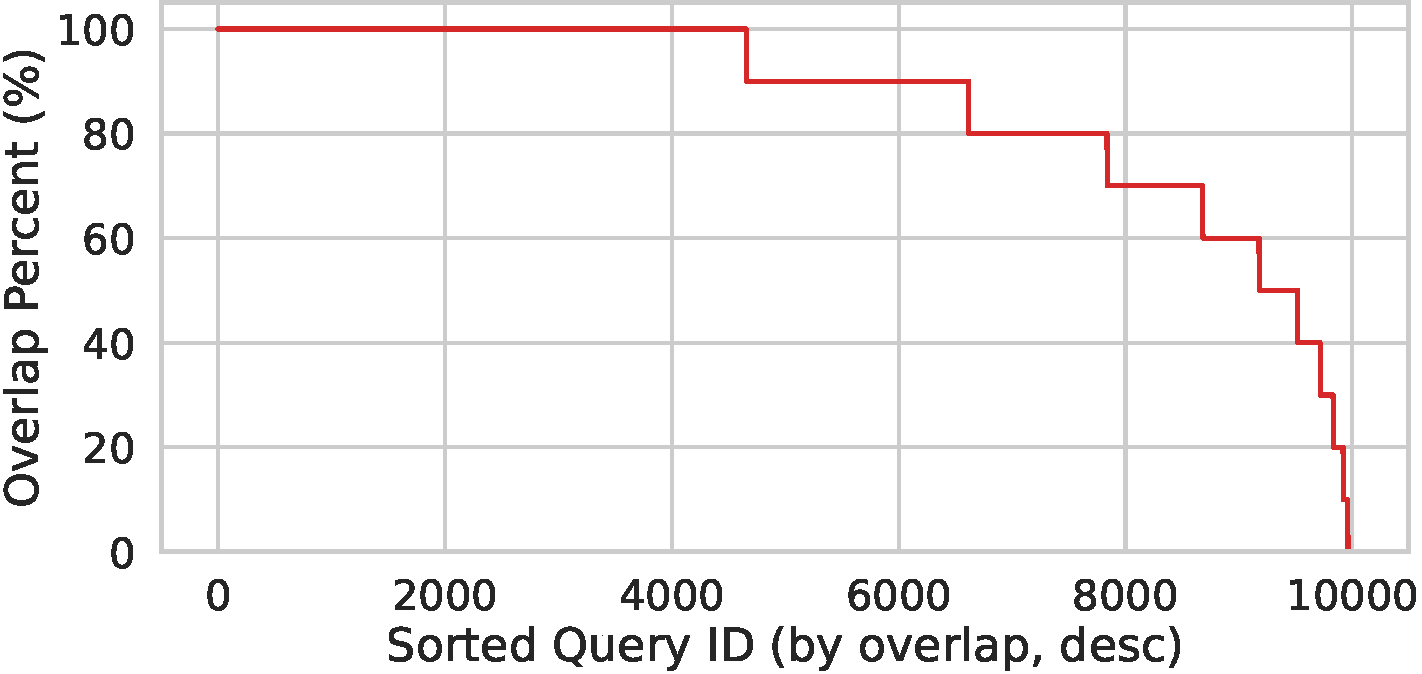
\includegraphics[width=0.7\columnwidth]{figures/query_overlap_set_desc_batch4_vs_batch5.pdf}
    \label{fig:per-query difference}
  }
    \caption{Key observations in dynamic ANNS workloads (HNSW, \texttt{SIFT}).}
	\label{fig:observation}
\end{figure*}


\noindent\textbf{Definition 1 (ANNS).}
Given a vector dataset $\mathcal{D}\subset\mathbb{R}^d$, a query $q\in\mathbb{R}^d$, and an integer $k$, ANNS returns an approximate top-$k$ set $\widehat{N}_k(q)$ that approximates the exact nearest-neighbor set $N_k^{\ast}(q)$ under a given distance metric. The search quality metric is $\mathrm{Recall@}k$:
\begin{equation}
\mathrm{Recall@}k(q)=\frac{|\widehat{N}_k(q)\cap N_k^{\ast}(q)|}{k}.
\end{equation}

Definition 1 captures the static setting, where the index remains fixed during queries. 
In the real world, however, vectors are continuously inserted, causing the ANNS index to evolve over time. 
To model this setting, we adopt the \textit{serialized round-based execution} model used in CANDOR-Bench~\cite{Wang202627}.

\noindent\textbf{Definition 2 (Dynamic ANNS).}
Dynamic ANNS operates as a sequence of update-query rounds. At each round $r$, the system first applies a batch of updates $\mathcal{U}_r$ to transform the previous dataset $\mathcal{D}_{r-1}$ into $\mathcal{D}_r$, and then executes a batch of queries $\mathcal{Q}_r$ on $\mathcal{D}_r$. The index structure is updated online across rounds.

In this setting, many optimizations developed for static ANNS become less effective as updates accumulate. As their effectiveness decays, query throughput drops and recall may also deteriorate. Frequent re-optimization is not a viable
solution either, because its maintenance overhead can dominate end-to-end cost, as shown in Figure~\ref{fig:reopt-cost}. This dilemma motivates the following problem.


\noindent\textbf{Problem Statement.}
Our goal is to maximize end-to-end query throughput under continuous updates, while preserving search quality comparable to the baselines. Since query acceleration is useful only when its maintenance overhead is affordable, we account for both query execution time and update-triggered maintenance time. Over $R$ update-query rounds, we measure end-to-end query throughput as:
\begin{equation}
\mathrm{QPS}(R) =
\frac{\sum_{r=1}^{R} |\mathcal{Q}_r|}
{
\sum_{r=1}^{R}\sum_{q\in\mathcal{Q}_r} T_{\mathrm{search}}(q)
+
\sum_{r=1}^{R} T_{\mathrm{maintain}}(\mathcal{U}_r)
}.
\end{equation}
where $T_{\mathrm{search}}(q)$ denotes the execution time of query $q$, and $T_{\mathrm{maintain}}(\mathcal{U}_r)$ denotes the maintenance time triggered by $\mathcal{U}_r$.

%In dynamic ANNS, low query latency is meaningful only if the maintenance required to sustain it is also affordable. We therefore account for both search time and maintenance time in the end-to-end throughput objective across update-query rounds.

%Let $\mathcal{Q}_r$ denote the query batch at round $r$, and let $n_r = |\mathcal{Q}_r|$ be the number of queries in that round. Over an evaluation horizon of $R$ rounds, we define the total search and total maintenance time costs as
%\begin{equation}
%T_s(R)=\sum_{r=1}^{R}\sum_{q\in\mathcal{Q}_r} T_{\mathrm{search}}(q), \quad T_m(R)=\sum_{r=1}^{R} T_{\mathrm{maintain}}(\mathcal{U}_r).
%\end{equation}
%The corresponding query throughput is
%\begin{equation}
%\mathrm{QPS}(R)=\frac{\sum_{r=1}^{R} n_r}{T_s(R)+T_m(R)}.
%\end{equation}
Accordingly, the optimization objective is to maximize $\mathrm{QPS}(R)$ subject to an average recall constraint:
\begin{equation}
\max \ \mathrm{QPS}(R)
\quad
\text{s.t.} \quad
\overline{\mathrm{Recall@}k}
\ge
\tau \cdot \overline{\mathrm{Recall@}k}^{\mathrm{baseline}}.
\end{equation}
where $\overline{\mathrm{Recall@}k}$ is the average recall over all queries in the $R$ rounds, and $\tau \in (0,1]$ specifies the required recall ratio relative to the baseline. We set $\tau=0.98$ in our experiments. More workloads may be evaluated in the future.

% \begin{equation}
% \begin{aligned}
% \max \quad & \mathrm{QPS}(R) \\
% \text{s.t.}\quad &
% \frac{1}{\sum_{r=1}^{R} n_r}
% \sum_{r=1}^{R}\sum_{q\in\mathcal{Q}_r}\mathrm{Recall@}k(q)
% \ge
% \tau \cdot \overline{\mathrm{Recall}}^{\mathrm{baseline}},
% \end{aligned}
% \end{equation}
% where
% \begin{equation}
% \overline{\mathrm{Recall}}^{\mathrm{baseline}}=
% \frac{1}{\sum_{r=1}^{R} n_r}
% \sum_{r=1}^{R}\sum_{q\in\mathcal{Q}_r}\mathrm{Recall@}k(q)^{\mathrm{baseline}},
% \end{equation}
% and $\tau \in (0,1]$ controls the required recall ratio relative to the baseline.




\subsection{Key Observations}

We perform a preliminary study of dynamic ANNS workloads using HNSW as a case study and summarize three observations.

\noindent\textbf{Observation 1: Recent search outcomes often remain informative across consecutive rounds.} For the same query batch, the top-$k$ results often remain highly overlapping across consecutive update rounds. 
As shown in Figure~\ref{fig:repeat results}, the 
overlap ratio of top-$k$ results quickly exceeds 80\% after the first few batches and remains around 95\% thereafter. This result suggests that the applied updates do not immediately cause large 
changes in the query results. Therefore, recent high-quality search results can still provide useful guidance for later queries, even though they should not be blindly returned as final answers.



\noindent\textbf{Observation 2: Returned vector frequencies are highly skewed.}
Across batch queries, the vector IDs appearing in top-$k$ results are not uniformly distributed. As shown in Figure~\ref{fig:skewness}, a small fraction of vectors appears frequently in query results, while most vectors are rarely returned.
This skew suggests that historical search results are not equally useful: prioritizing results related to frequently returned vectors is likely to provide more benefit than treating all past outcomes uniformly.

%As shown in Figure~\ref{fig:skewness}, the frequency of hit node IDs follows a clear long-tail distribution: a small fraction of IDs is found very frequently, while the majority is rarely observed. This skew indicates that query-hit patterns in dynamic ANNS are highly uneven, and that not all recurring search outcomes are equally valuable for reuse. As a result, treating historical outcomes discriminately is likely to be cost-effective.

\noindent\textbf{Observation 3: Result stability varies across queries.}
Within a query batch, different queries can respond very differently to updates. Figure~\ref{fig:per-query difference} shows that roughly 45\% of queries keep
their top-$k$ results unchanged before and after batch updates, while nearly 10\% of queries experience at least 50\% changes in their top-$k$ results. This variation suggests that historical results cannot be assumed to be reliable for all queries, even when the overall batch-level overlap remains high.


\subsection{Design Challenges}

Although the observations above reveal clear opportunities for dynamic ANNS acceleration, exploiting them efficiently and robustly under continuous updates remains non-trivial,
with the following challenges:

\noindent\textbf{Challenge 1: How to store and represent historical search results?}
Observation 1 shows that recent top-$k$ results can remain stable across nearby update rounds.
However, storing complete query results for all past queries is neither memory-efficient nor necessary.
The system must decide what information from previous queries should be stored, how to represent it in a compact form, and how to attach simple signals that reflect its freshness and usefulness.
It must also support bounded retention and eviction, so that outdated or low-value records do not accumulate as updates continue.








%Although Observation 1 suggests that recent top-$k$ results can remain useful across nearby update rounds, high overlap does not imply that past outcomes can be reused unchanged. Instead, they should be retained as lightweight guidance for future search. Therefore, the system must decide what information should be preserved from previous queries, how to represent it compactly, and how to store it under bounded memory overhead. Moreover, it must also balance retention and eviction so that useful outcomes remain available while stale ones are removed over time.

\noindent\textbf{Challenge 2: How to guide new queries with stored results?}
Stored historical results are useful only if they can be matched to later queries and used to reduce search cost.
This is straightforward when a query repeats a previous one, but harder when the query is only similar to past queries.
The system must therefore decide which stored results are relevant to the current query and how they can guide the current search.
Observation 2 further shows that returned vector frequencies are highly skewed, approximately following a Zipf distribution with an exponent of 1.167, indicating that stored results should not be treated uniformly during retrieval and reuse.

%Even when historical outcomes are stored, turning them into effective search guidance remains non-trivial. The system must activate relevant outcomes for queries that do not exactly match previous ones, and use them to recover strong candidates without causing excessive search expansion. Moreover, Observation 2 suggests that reuse should be selective rather than uniform: highly recurring outcomes and long-tail outcomes may need to be handled differently in order to achieve good performance under bounded cost. But, how to design such a selective reuse mechanism that can adapt to changing query-hit patterns is an open question.

\noindent\textbf{Challenge 3: How to validate the new results derived from stored results?}
Even if historical search results can be retrieved for a new query, the results derived from them may not be reliable after updates.
Observation 3 shows that result stability varies significantly across queries, so blindly trusting stored results can lead to degraded search quality, with recall deviations of up to 0.81\%.
The system must decide whether to accept the generated top-$k$ results or fall back to the original search path.
This validation step must be lightweight; otherwise, its cost can offset the benefit of reusing stored results.

%Even when historical outcomes are well represented and selectively prioritized for search, reuse does not automatically improve both overall performance and recall, because the identified historical outcomes may still be unreliable for current search. The system must therefore decide whether the reused search path should be accepted or whether it should fall back to the native search path, while keeping this decision process sufficiently lightweight. Designing such an acceptance-and-fallback mechanism is critical to ensuring that historical-outcome reuse improves efficiency without degrading recall.

Motivated by these challenges, we next present \system and elaborate on how it addresses Challenges 1--3.